\section*{Problem 1 - Attitude Control of Satellite}

The objective of problem 1 is to control attitude of a Satellite. The satellites equations of motions are represented in equation \eqref{eq:dynamics}, equation ?? \todo{find number in fossen} \cite{Fossen2011}. The parameters for this specific Satellite are; $\mathbf{I}_{CG} = mr^2$, $m = 100 kg$, $r = 2.0 m$. 

\begin{subequations}
\label{eq:dynamics}
	\begin{align}
		\dot{\mathbf{q}} = \mathbf{T}_q (\mathbf{q} ) \boldsymbol{\omega} \\
		\mathbf{I}_{CG} \dot{\boldsymbol{\omega}} - \mathbf{S} (\mathbf{I}_{CG} \boldsymbol{\omega} ) \boldsymbol{\omega} & =  \boldsymbol{\tau} 
		\label{eq:EOM_omega_dot}
	\end{align}	
\end{subequations}

This equations uses the unit quaternions and Euler angles. The unit  quaternions are represented as $q = [\eta, \epsilon_1, \epsilon_2, \epsilon_3]^T$ and only the positive $\eta$ is used, leading to equations \eqref{eq:pos_eta}. The Euler angles are represented as $\theta = [\phi , \theta , \psi]^\top$ and their representative angular velocities are  $\omega = [\omega_1, \omega_2, \omega_3]$. In \cite{Fossen2011} $\omega$ is often written as $\omega = [p,q,r]$, but because of the parameter $r = 2.0m$, in this rapport $\omega$ is written as $[\omega_1, \omega_2, \omega_3]^\top$.

\begin{equation}
    \eta = \sqrt{1 - \epsilon^\top \epsilon} 
    \label{eq:pos_eta}
\end{equation}
 
In this lab rapport the state of the system $x = [ \boldsymbol{\epsilon}^T, \boldsymbol{\omega}^\top]$ and the input to the system $\mathbf{u} = \boldsymbol[0,0,0,\tau_1, \tau_2, \tau_3]^\top$. The reason for the upper three zeros in the input, is because of $\dot{\boldsymbol{\epsilon}}$ do not have any input, while $\dot{\boldsymbol{\omega}}$ have input $\boldsymbol{\tau}$.

\todo{Should we write introduction ?}

\subsection*{Problem 1.1}

\subsubsection*{Finding the equilibrium point}

The equilibrium point is defined as the steady-state solution of a system, meaning $\dot{\mathbf{x}} = 0$ with $\mathbf{x}$ being the state of the system.


The equilibrium point $\mathbf{x_0}$ of the closed-loop system $\mathbf{x} = [ \boldsymbol{\epsilon}^T, \boldsymbol{\omega}^T]^T$ corresponding to $\mathbf{q} = [\eta,\epsilon_1, \epsilon_2, \epsilon_3]^T = [1, 0, 0, 0]$ and $\boldsymbol{\tau} = \boldsymbol{0}$ may be found by setting $\dot{\boldsymbol{\epsilon}} = \mathbf{0}$ and $\dot{\boldsymbol{\omega}} = \mathbf{0}$. The equation for $\boldsymbol{\epsilon}$ and $\boldsymbol{\omega}$ may be found by using equation (2.86) in \cite{Fossen2011} and \eqref{eq:EOM_omega_dot}. From equation (2.86) in \cite{Fossen2011} and \eqref{eq:EOM_omega_dot} the following equations was found:


\begin{subequations}
\label{eq:x_dot}
	\begin{align}
		\dot{\boldsymbol{\epsilon}} =  [ \eta \mathbf{I}_{3X3} + \mathbf{S}(\boldsymbol{\epsilon}) ] \boldsymbol{\omega}  \label{eq:episilon_dot} \\
		 \dot{\boldsymbol{\omega}} = \mathbf{I}_{CG}^{-1} [\mathbf{S} (\mathbf{I}_{CG} \boldsymbol{\omega} ) \boldsymbol{\omega} +  \boldsymbol{\tau} ] \label{eq:omega_dot}
	\end{align}	
\end{subequations}

\todo{Write top instead of T }
\todo{Should I take in equation 2.68 ?}

With $\mathbf{S} (\boldsymbol{\epsilon})$ and being the skewmatrix $\mathbf{S} (\mathbf{I}_{CG} \boldsymbol{\omega} ) $, as defined in \cite{Fossen2011} equation ???? \todo{need to find reference} . Equation \eqref{eq:episilon_dot} may be written as:

\begin{equation}
    \begin{aligned}
	\dot{\boldsymbol{\epsilon}}
	&= 
	\left \{
	\begin{bmatrix}
		\sqrt{1-\boldsymbol{\epsilon}^\top \boldsymbol{\epsilon}} & 0 &  0  \\
		0 & \sqrt{1-\boldsymbol{\epsilon}^\top \boldsymbol{\epsilon}} &   0   \\
		0 &  0  & \sqrt{1-\boldsymbol{\epsilon}^\top \boldsymbol{\epsilon}} 
	\end{bmatrix}
	+
	\begin{bmatrix}
		0 & -\epsilon_3 &  \epsilon_2   \\
		\epsilon_3 & 0 &   - \epsilon_1   \\
		-\epsilon_2 &  \epsilon_1  & 0
	\end{bmatrix}
	\right \} 
	\begin{bmatrix}
		\omega_1  \\
		\omega_2  \\
		\omega_3  \\
	\end{bmatrix}
	\end{aligned}
	\label{eq:epsilon_dot_full}
\end{equation}

By using equation \eqref{eq:epsilon_dot_full},   $\mathbf{q} = [1, 0, 0, 0]^\top$ and $\boldsymbol{\tau} = \boldsymbol{0}$ the equilibrium point $\mathbf{x} = [0, 0, 0, 0]^\top$. Since equation \eqref{eq:epsilon_dot_full} have 3 unkonwn parameters and 3 equations, it was not needed to include equation \eqref{eq:omega_dot}. Another problem with using equation \eqref{eq:omega_dot} is that by using the constraints  $\mathbf{q} = [1, 0, 0, 0]^\top$ and $\boldsymbol{\tau} = \boldsymbol{0}$ gives only 2 equations, and 3 unkonwn parameters ( $\omega_1, \omega_2, \omega_3$).

\todo{Should we write more about the calculations?}

\subsubsection*{Linearize the equations of motion}

A general linearized model is $ \Delta \dot{\mathbf{x}} = \mathbf{A} \Delta \mathbf{x} + \mathbf{B} \Delta \mathbf{u}$. $\Delta \mathbf{x} = \mathbf{x} - \mathbf{x}_0$ are the linearized coordinate transformed states of the system and $\Delta \mathbf{u} = \mathbf{u} - \mathbf{u}_0$ are the corresponding coordinate transformed input. 

A system of the form $\dot{\mathbf{x}} = f(\mathbf{x , u})$, may be linearized by using \eqref{eq:Jocobians}. In equation \eqref{eq:Jocobians} the matrices \textbf{A} and \textbf{B} of the linearized system is calculated by using the Jacobians of $f(\mathbf{x,\boldsymbol{\tau}}$, and the equlibrium point. 

\begin{equation}
    \begin{aligned}
        \mathbf{A}&= \frac{\partial f(\mathbf{x,\boldsymbol{\tau}})}{\partial \mathbf{x}}\Bigr|_{\substack{\mathbf{x}= \mathbf{x}_0 \\ \boldsymbol{\tau=0 }}} &
        \mathbf{B}&= \frac{\partial f(\mathbf{x,\boldsymbol{\tau}})}{\partial \mathbf{u}}\Bigr|_{\substack{\mathbf{x}= \mathbf{x}_0 \\ \boldsymbol{\tau=0 }}} 
    \end{aligned}
    \label{eq:Jocobians}
\end{equation}

The equation of motion of the satellite , equation \eqref{eq:x_dot}, represented as a function of the form $\dot{\mathbf{x}} = f(\mathbf{x , u})$ are:

\begin{equation}
    \begin{aligned}
    \begin{bmatrix}
		\dot{\boldsymbol{\epsilon}} \\
		\dot{\boldsymbol{\omega}}
    \end{bmatrix}
    &=
	\mathbf{f(\mathbf{x},t)} 
	&= 
	\begin{bmatrix}
		\frac{1}{2}[ \sqrt{1-\boldsymbol{\epsilon}^\top \boldsymbol{\epsilon}} \omega_1  - \epsilon_3 \omega_2 + \epsilon_2 \omega_3  ] \\
		\frac{1}{2}[ \epsilon_1 \omega_3 +  \sqrt{1-\boldsymbol{\epsilon}^\top \boldsymbol{\epsilon}} \omega_2  - \epsilon_1 \omega_3 ] \\
		\frac{1}{2}[  - \epsilon_2 \omega_1  + \epsilon_1 \omega_2 + \sqrt{1-\boldsymbol{\epsilon}^\top \boldsymbol{\epsilon}} \omega_3  ] \\
		\tau_1 \frac{1}{mr^2}\\
		\tau_2 \frac{1}{mr^2}\\
		\tau_3 \frac{1}{mr^2}\\
	\end{bmatrix}
	\label{eq:f}
	\end{aligned}
\end{equation}


The linearized  closed-loop system was calculated using equation \eqref{eq:f} , \eqref{eq:Jocobians} and equilibrium point $\mathbf{x}_0 = [0,0,0,0,0,0]$ and $\mathbf{u} = [0,0,0,0,0,0]$. The lineariezd system $\Delta \dot{\mathbf{x}} = \mathbf{A}\Delta \mathbf{x} + \mathbf{Bu}$ , with matrixes $\mathbf{A}$ and $\mathbf{B}$ are represtented in equation \eqref{eq:linearized_sys_matrices} :


\begin{equation}
    \begin{aligned}
	\mathbf{A}
	&=
	\begin{bmatrix}
		0 & 0 & 0 & \frac{1}{2} & 0   & 0\\
		0 & 0 & 0 & 0   & \frac{1}{2} & 0\\
		0 & 0 & 0 & 0   & 0   & \frac{1}{2}\\
		0 & 0 & 0 & 0 & 0 & 0\\
		0 & 0 & 0 & 0 & 0 & 0\\
		0 & 0 & 0 & 0 & 0 & 0\\
	\end{bmatrix}
	&
	\mathbf{B}& = 
	\begin{bmatrix}
		0 & 0 & 0 & 0 & 0 & 0\\
		0 & 0 & 0 & 0 & 0 & 0\\
		0 & 0 & 0 & 0 & 0 & 0\\
		0 & 0 & 0 & \frac{1}{400} & 0 & 0\\
		0 & 0 & 0 & 0 & \frac{1}{400} & 0\\
		0 & 0 & 0 & 0 & 0 & \frac{1}{400}\\
	\end{bmatrix}
	\end{aligned}
	\label{eq:linearized_sys_matrices}
\end{equation}

\todo{write in Delta}

\subsection*{Problem 1.2}
In this problem the following control law is suggested for for controlling the satellite  
\begin{equation}
  \mathbf{\tau} = -\mathbf{K}_d \boldsymbol{\omega} - k_p \boldsymbol{\epsilon}
  \label{eq:control_1}
\end{equation}

with $\mathbf{K}_d = k_d \mathbf{I}_{3x3}$ , $k_d = 20$ and $k_p = 1$.  

\subsubsection*{Analysis of linarized system stability}

The stability of the linearized system may be analysed by looking at the placement of the poles of the system.

The control law represented in equation \eqref{eq:control_1} may be represented on the form $ \mathbf{u} = - \mathbf{K} \mathbf{x}$. The input to the system using control law from equation \eqref{eq:control_1} is:

\begin{equation}
\begin{aligned}
    \mathbf{K}
    &=
    \begin{bmatrix}
    0 & 0 & 0 & 0 & 0 & 0 \\ 
    0 & 0 & 0 & 0 & 0 & 0 \\ 
    0 & 0 & 0 & 0 & 0 & 0 \\ 
    k_p & 0 & 0 & k_d & 0 & 0 \\ 
    0 & k_p & 0 & 0 & k_d & 0 \\ 
    0 & 0 & k_p & 0 & 0 & k_d \\ 
    \end{bmatrix}
    \label{eq:K}
\end{aligned}
\end{equation}

The linearized system is on the form $\Delta \mathbf{x} = \mathbf{A}\Delta \mathbf{x} + \mathbf{B} \Delta \mathbf{u}$, may with the control law in equation \eqref{eq:control_1} be written as $\Delta \dot{\mathbf{x}} = \mathbf{A}\Delta \mathbf{x} - \mathbf{B K} \Delta \mathbf{x} = ( \mathbf{A}\Delta  - \mathbf{B K} ) \Delta \mathbf{x} $.

The poles of the system may be found by calculating the eigenvalues of $( \mathbf{A}\Delta  - \mathbf{B K} )$. The calculation of the eigenvalues was done by using the \texttt{MATLAB}-function \texttt{lambda = eig(A)}, with lambda being a vector of the eigenvalues of A. The functionality of finding the eigenvalues of the closed-loop system with control-law given in \eqref{eq:control_1} is implemented in the file
{\color{blue}  stability\_system.m }. The eigenvalues are = $- 0.0250 \pm 0.0250i$, where 3 poles are corresponding . Since the real part of the eigenvalues are negative, the system is stable.

\subsubsection*{Discussion real or imaginary poles}

When placing poles were are multiple considerations to consider. Most likely you would want your system to be stable, meaning the poles of the system should be placed in the left half-plane. Real poles gives exponentially decaing components, where the rate is increases the more negative the poles are. While a complex conjugate pole pair in the left-half of the s-plane combines to generate a response component that is a decaying sinusoid. The rate of decay is specified by the real-part of the pole and the frequency is descided by the imaginary-part of the pole. This means a system with real-poles in left-half plane will steadly reach the correct value, while an imaginary poles in left-half plane may reach steady-state value faster than a real-pole but to the cost of stability. A system having one or more poles lying on the imaginary axis of the s-plane has non-decaying oscillatory components in its homogeneous response. In space this seams like a not wanted response in the system, because of less interrupting forces, like friction. 

When choosing poles, the most important thing is to look into the dynamics of the system. Each pole effects a different part of the system.  

Genereally since the satellite is in space, it should not have to big oscillations because of less interrupting forces. At the same time, with real poles as fast as complex-poles need more power, which a satellite may not have and may lead to more saturation.

Since the satellite should be relatively fast, and do not have that much power it is suggested to have imaginary poles, with small oscillatory parts. This suggestion will lead to a bit faster satellite, which will save the satellite some power but to the expence of some less stability.  

\subsection*{Problem 1.3}
\subsubsection*{Simmulation of system with simple controller}

In {\color{blue}  attitude1.m } the system is simmulated with a controller based on the the control law from \eqref{eq:control_1}. This is done by using a for-loop initialized with Euler-parameters $\phi = 10 \circ$, $\theta = -5 \circ$ and $\psi = 15  \circ$. To initializa the unit quaternion-parameters the \texttt{MATLAB}-function \texttt{q = euler2q(phi,theta,psi)} from the library \texttt{MSS} was used. The function transforms from euler-coordiantes to unit quaternions. The angular velocity $\boldsymbol{\omega}$ is initalized to $\mathbf{0}$. 

In the simulation for-loop first the input to the system is calculated based on last iteration states, based on the linarized system with $\mathbf{u} = -\mathbf{K}\mathbf{x}$, with K from \eqref{eq:K}.  From the equation of motion , \eqref{eq:x_dot}, $\dot{\mathbf{x}}$ is calculated. The next state is estimated by using Euler integration on quaternion-coordinates $\mathbf{q}$ and the angular velocities $\mathbf{omega}$. Before the quaternions are normalized, such that it is unit quaternions. The euler-coordinates, unit quaternions and angular-velocities are saved in a variable table, used for plotting.

The result after the plotting are represented in Figure \ref{fig:sim_attitude1_euler} - \ref{fig:sim_attitude1_tau}. 

\begin{figure}[htb!]
	\centering
	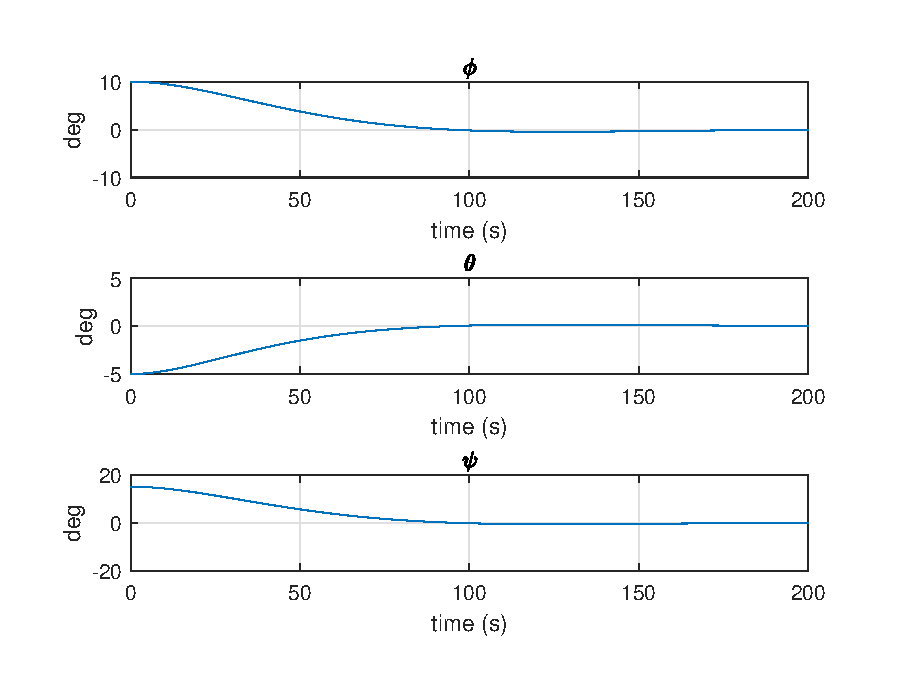
\includegraphics[width=1.00\textwidth]{figures/1_euler.eps}
	\caption{The resulting output Euler angles from the simulation in attitude1.m}
\label{fig:sim_attitude1_euler}
\end{figure}

\begin{figure}[htb!]
	\centering
	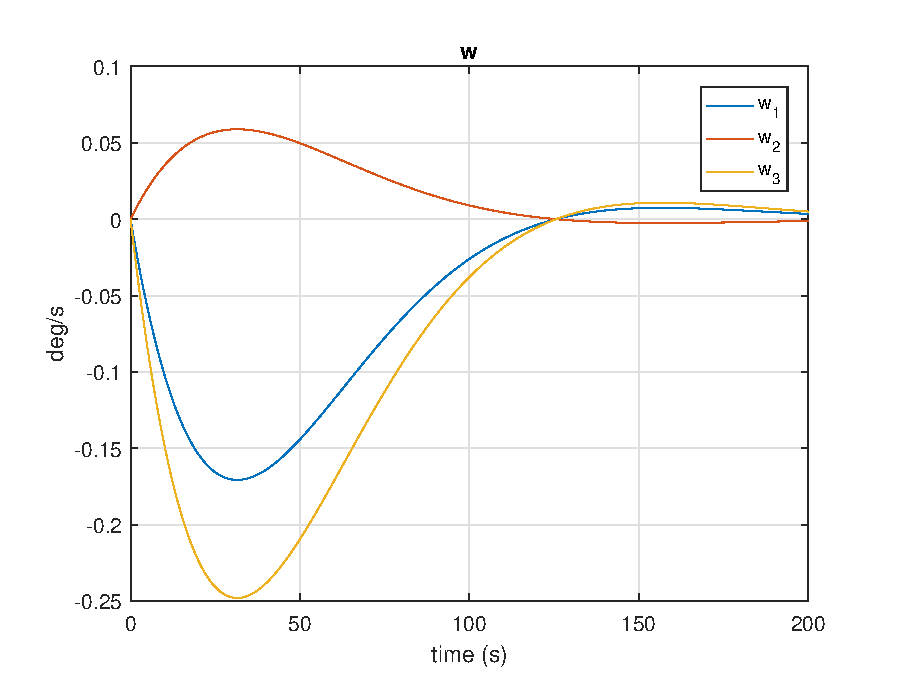
\includegraphics[width=1.00\textwidth]{figures/1_q.eps}
	\caption{The resulting state $x = [\boldsymbol{\eta}^\top, \boldsymbol{\omega}^\top] ^\top$ of the system and $\eta$. $\boldsymbol{\omega}$ is \textbf{w} in the figure. The figure is from the simulation in attitude1.m}
\label{fig:sim_attitude1_q}
\end{figure}

\begin{figure}[htb!]
	\centering
	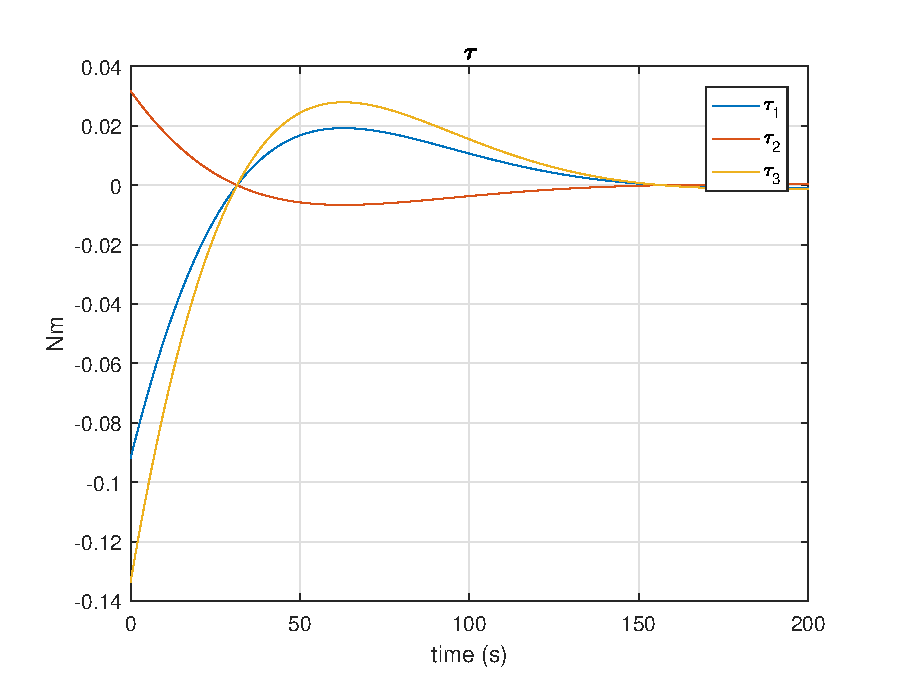
\includegraphics[width=1.00\textwidth]{figures/1_tau_track.eps}
	\caption{The resulting input , $\boldsymbol{\tau}$from the simulation in attitude1.m}
\label{fig:sim_attitude1_tau}
\end{figure}

\todo{Skrives Euler med store eller små bokstaver ?}





